\documentclass{article}%
\usepackage[T1]{fontenc}%
\usepackage[utf8]{inputenc}%
\usepackage{lmodern}%
\usepackage{textcomp}%
\usepackage{lastpage}%
\usepackage{geometry}%
\geometry{left=3cm,right=3cm,bottom=2cm,top=1cm}%
\usepackage[russian]{babel}%
\usepackage{amsmath}%
\usepackage{amssymb}%
\usepackage{amsfonts}%
\usepackage{mathtext}%
\usepackage{graphicx}%
%
%
%
\begin{document}%
\normalsize%
\begin{center}%
.\\%
\vspace{12cm}%
\textbf{Лабораторная работа № 3.13: Магнитное поле Земли}%
\end{center}%
\begin{center}%
Исхаков Камиль Фархатович%
\end{center}%
\begin{center}%
\today%
\end{center}%
\newpage%
\section{Основные формулы:}%
\label{sec:}%

%
Отношение между направлениями пробного поля и земного магнитного поля:\begin{displaymath}{\frac{\sin{\alpha}}{\sin{\phi-\alpha}}} = {\frac{B_h}{B_c}}\end{displaymath}%
\newline%
где $B_h, B_c$ – направления пробного поля и земного магнитного поля соответственно; $\phi$ – угол между $B_c$ и $B_h$, а $\alpha$ – угол между направлением результирующего поля и земного магнитного поля.%
\newline%
Величина магнитной индукции на оси одного кругового тока:\begin{displaymath}B(x) = \frac{\mu_0 I}{2} \frac{R^2}{(x^2+R^2)^{3/2}}\end{displaymath}%
\newline%
где $I$ – сила тока, $R$ – средний радиус каждой катушки,$\mu_0$ – магнитная постоянная, $x$ – расстояние от центра контура%
\newline%
Модуль вектора направления пробного поля:\begin{displaymath}B_c = \mu_0 \left(\frac{4}{5}\right)^{3/2} \frac{I n}{R}\end{displaymath}%
\newline%
где $n$ – число витков в каждой катушке%
\newline%
\section{Расчеты:}%
\label{sec:}%

%


\begin{table}[h!]%
\caption{Результаты прямых измерений}%
\begin{tabular}{|c|c|c|c|c|c|}%
\hline%
$\varphi = \ldots^\circ$&\multicolumn{3}{|c|}{Ток в катушках, мА}&&\\%
\hline%
$\alpha_i$&$I_1$&$I_2$&$\langle I \rangle$&$\frac{\sin (\alpha_i)}{\sin (\varphi - \alpha_i)}$&$B_c, \text{мкТл}$\\%
\hline%
10°&6.40&7.70&7.05&0.36&4.23\\%
\hline%
20°&12.50&12.60&12.55&0.54&7.52\\%
\hline%
30°&15.00&16.00&15.50&0.66&9.29\\%
\hline%
40°&17.70&18.20&17.95&0.75&10.76\\%
\hline%
50°&19.40&19.40&19.40&0.82&11.63\\%
\hline%
60°&21.10&20.40&20.75&0.88&12.44\\%
\hline%
70°&21.90&22.30&22.10&0.94&13.25\\%
\hline%
80°&23.20&23.60&23.40&1.00&14.03\\%
\hline%
90°&25.20&25.10&25.15&1.06&15.08\\%
\hline%
100°&26.30&26.30&26.30&1.13&15.77\\%
\hline%
110°&28.90&28.20&28.55&1.21&17.11\\%
\hline%
120°&30.80&30.30&30.55&1.32&18.31\\%
\hline%
130°&33.70&33.80&33.75&1.49&20.23\\%
\hline%
140°&40.90&39.50&40.20&1.79&24.10\\%
\hline%
\end{tabular}%
\end{table}

%
\newpage%


\begin{figure}%
\centering%
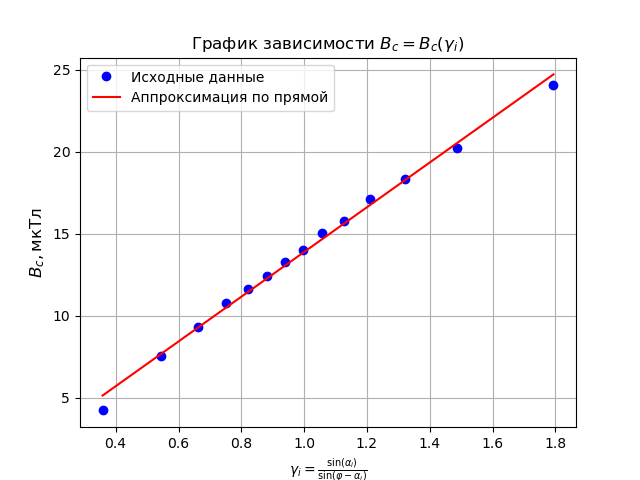
\includegraphics[width=350px]{linear_approximation.png}%
\end{figure}

%
Угловой коэффициент  a = 13.6500 мкТл, что должно соответствовать величине магнитного поля Земли. Из методического пособия А.Ф. Костко В.А. Самолетов 'ФИЗИКА ЛАБОРАТОРНЫЕ РАБОТЫ ПО ЭЛЕКТРИЧЕСТВУ И МАГНЕТИЗМУ', можно получить информацию о том, какова величина магнитного поля Земли в Санкт-Петербурге, которая равна 15,4 мкТл. Найдем погрешность углового коэффициента, а также доверительный интервал при $\alpha = 0.95$:\vspace{0.5cm}\\\textbf{Погрешность углового коэффициента}:  $\pm$0.6239 мкТл\vspace{0.5cm} \\\textbf{Доверительный интервал} для $95.0\%$: 13.6500 $\pm$2.1788 мкТл\vspace{0.5cm}%
\newline%
\section{Выводы}%
\label{sec:}%

%
Во время выполнения лабораторной работы удалось установить диапазон величины магнитного поля Земли, в котором содержится истинное ее значение.Также была сделана линейная аппроксимация данных, которая хорошо описывает зависимость.Коэффициенты линейной аппроксимации: a = 13.6500, b = 0.2400%
\newline%
\end{document}